
\begin{frame}[fragile]{Démonstration de l'application ``transactions''}

Exécution en concurrence  de deux transactions de réservation, 
$T_g$ (à gauche) et  $T_d$ (à droite)

\vfill
\begin{center}
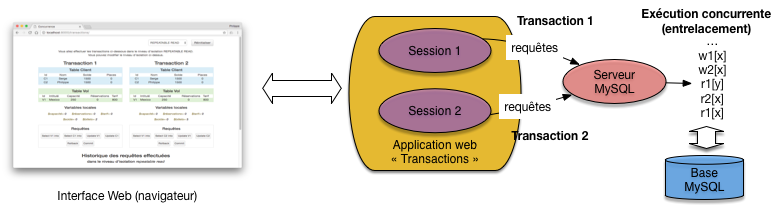
\includegraphics[width=10cm]{../../figures/demo-transactions}
\end{center}


\vfill

\begin{blocgauche}
\`A tester\,: \url{http://deptfod.cnam.fr/bd/tp/}
\end{blocgauche}


\end{frame}

%%%%
\begin{frame}{Scénario 1\,: l'isolation}


\vfill 

\begin{redbullet}
  \item $T_g$ lit et modifie le vol
  \item  $T_d$ lit le vol et ne voit pas de changement
  \item $T_g$ lit le vol et voit ses changements
  \item $T_g$ valide\,: celle de droite ne voit rien
  \item  $T_d$ valide pour débuter une nouvelle transaction\,:
      les changements deviennent visibles 
\end{redbullet}

\vfill

\alert{Conclusion}\,: une transaction voit toujours la base telle qu'elle était
au moment où elle a commencé.
\end{frame}


%%%%
\begin{frame}{Scénario 2\,: atomicité et durabilité}

\vfill 

\begin{redbullet}
  \item $T_g$ lit et modifie le vol et le client
  \item  $T_d$  ne voit pas de changement
  \item $T_g$ annule avec \sqlkw{rollback}
  \item Les deux transactions peuvent voir les données initiales
  \item On recommence, mais avec \sqlkw{commit}, puis \sqlkw{rollback}. Le \sqlkw{rollback}
     n'a plus aucun effet
\end{redbullet}

\vfill

\alert{Conclusion}\,: il est possible à tout moment d'annuler avec \sqlkw{rollback}, 
jusqu'au \sqlkw{commit} qui lui, est définitif.
\end{frame}


%%%%
\begin{frame}{Scénario 3\,: la cohérence}

\vfill 

\begin{redbullet}
  \item $T_g$ effectue lectures puis écritures, puis \sqlkw{commit}
  \item Idem pour  $T_d$: la base est toujours cohérente
  \item $T_g$ effectue les lectures, idem pour  $T_d$
  \item $T_g$ effectue les écritures, idem pour  $T_d$
  \item \alert{La base est incohérente}
\end{redbullet}

\vfill

\alert{Conclusion}\,: une exécution \alert{en série} ne pose jamais de problème;
une exécution \alert{concurrente} peut mener à des anomalies.
\end{frame}


\begin{frame}{Scénario 4\,: verrouillages et interblocages}

\begin{redbullet}
  \item $T_g$ effectue lectures puis écritures
  \item  $T_d$ effectue lectures puis écritures: mise en attente
\end{redbullet}

\alert{Conclusion}\,: les lectures sont concurrentes, pas les écritures

\vfill

Maintenant on se place en mode \sqlkw{serializable}

\begin{redbullet}
  \item $T_g$ effectue les lectures, idem pour  $T_d$
  \item $T_g$ effectue les écritures, idem pour  $T_d$\,: blocage complet
\end{redbullet}

\vfill

\alert{Conclusion}\,: si on veut l'isolation complète, on prend le risque d'un interblocage.

\end{frame}


\begin{frame}{Résumé}

La démonstration a montré les principales propriétés des transactions concurrentes 

\vfill 

\begin{redbullet}
  \item Les MAJ effectuées par une transaction sont visibles par cette même transaction
  \item Les MAJ effectuées par une transaction, et pas encore validées, ne sont pas visibles des autres transactions
   \item Le \sqlkw{commit} rend les mises à jour irréversibles\,; le \sqlkw{rollback} les annule
   \item Le niveau d'isolation est paramétrable\,; seul le plus élevé garantit la cohérence.
\end{redbullet}

\end{frame}
